\newpage
\section{Aufgabe 2}
Zur Ermittlung der Position des Moskitos wird dessen Fluggeräusch mit vier Mikrofonen gleichzeitig abgetastet.
Dabei wird das Signal mit 48kHz bzw. 96kHz abgetastet. 
Der Empfänger zeichnet gleichzeitig die empfangenen Signale an allen vier Mikrofonen auf. 
Anhand der empfangenen Signalen werden die relativen Laufzeitverzögerungen zwischen den Mikrofonen berechnet und darüber anschließend die Position mit dem bereits erklärten "Newton-Verfahren" ermittelt. Um dabei die Effizienz der Berechnung zu erhöhen, werden die von den Mikrofonen aufgezeichneten Signale gekürzt, diese gekürzten Signale bilden dabei die Hauptsignale. 
Die relativen Verzögerungen werden dadurch ermittelt, dass die Hauptsignale mit einem aus dem Hauptsignal herausgeschnittenen Teilsignal, dem Korrelationssignal, korreliert. Durch die Korrelation eines Teilsignals mit den vier Hauptsignalen lässt sich jeweils die Position des Teilsignals in den Hauptsignalen ermitteln. Anhand der Position lässt sich wiederrum die relative Verzögerung ermitteln. \\
Wie die Signale gekürzt werden, um die wichtigsten Merkmale zu erhalten und dennoch eine beringe Berechnungsdauer gewehrleisten zu können wird im folgenden geklärt.
\\ Zur Vereinfachung werden hier vorerst lediglich die Signale von zwei Mikrofonen betrachtet. 
\subsection{Herrauslösen der Hauptsignale} \label{sec:Eins}
Da die Mikrofone zeitgleich das Signal des Moskitos aufzeichnen, kommt es aufgrund der Laufzeitunterschiede des Signals zu einer Verschiebung der Signalwerte in den empfangenen Signalen untereinander. \\
So empfängt beispielsweise MIC1 den Signalabschnitt $X$ nach 10ms, wohingegen MIC2 aufgrund der größeren Entfernung zum Moskito den selben Abschnitt $X$ erst nach 20ms empfängt.\\
Beginnt man nun beim Herrauslösen der Hauptsignale am Anfang des empfangenen Signals führt dies dazu, dass Mikrofone die näher am Moskito sind diese gar nicht empfangen haben. Dies hat zur Folge, dass die Laufzeitdifferenz nicht korrekt ermittelt werden kann, da die Korrelation keine korrekten Ergebnisse liefern kann.\\
Um diesem Fehlerfall entgegenzu wirken, dürfen die Hauptsignale erst nach einem "Totbereich" herrausgelöst werden. Die Dauer des Totbereiches $t_{min}$ wird dabei über den maximal möglichen Abstand $a_{max}$ der Mikrofone zueinander ermittelt:
$$	t_{min} = \frac{a_{max}}{c_{s}} = 3.57 ms$$
Über die $t_{min}$ und die SamplingRate $f_s$ lässt sich dabei die Größe des Totbereiches $K_{min}$ in der Indexierung des Singales errechnen:
\begin{equation}
	K_{min} = f_s * t_{min}   = f_s * \frac{a_{max}}{c_{s}} \label{eq:A2A2E1}
\end{equation}

Wird der selbe pyramidenförmige Mikrofonaufbau wie im ersten Teil des Praktikums verwendet, ergibt sich für den maximalen Abstand $a_{max}$ eine Distanz von von $a_{max} = \frac{\sqrt{6}}{2}m$. Mit einer SamplingRate von $f_s = 96 kHz$ folgt aus der Gleichung\eqref{eq:A2A2E1} ein Totbereich von $K_{min} \approx 343$. Um noch etwas Sicherheit einzubauen und Rundungsfehler auszugleichen wurde für das Matlab Programm ein Totbereich von $K_{min} = 500$ gewählt.

\subsection{Herrauslösen des Korrelationssignals}
Bei dem Korrelationssignal handelt es sich um einen Auszug aus dem Hauptsignal des ersten Mikrofons welcher als Referenz für die Korrelation mit den Signalen der anderen Mikrofone benutzt wird.\\
Ähnlich wie beim Herrauslösen der Hauptsignale ist auch hier darauf zu achten, dass das Korrelationssignal in den anderen Signalen enthalten ist. Da dies allerdings bereits bei dem Herrauslösen der Hauptsignale berücksichtigt wurde, bildet der erste Teil des Hauptsignal des ersten Mikrofons das Korrelationssignal. Es wird auf eine weitere Verschiebung des Teilsignals verzichtet, um die zu bearbeitende Datenmenge so klein wie möglich zu halten.


\subsection{Länge des Korrelationssignals $K_{corr}$}
Die Länge des Korrelationssignals $K_{corr}$ beieinflusst die Genauigkeit der Differenzmessung deutlich. Ist die Länge des Teilsignals zu kurz, ist keine genaue Positionsermittlung möglich, da es sein kann, dass die betrachteten Wertfolgen mehrmals in dem Hauptsignal auftauchen, bzw. verschwimmen. Durch die Verlängerung des Teilsignals wird dies verhindert und eine exaktere Positionsbestimmung mittels der Korrelation ist möglich. Längere Zeitsignale erhöhen allerdings den Rechenaufwand und damit die Rechendauer. \\
Als Richtwert wird dabei der Extremfall mit der maximal Möglichen Signalverschiebung angewendet. Dieser tritt auf, wenn sich der Moskito auf der Verbindungsgerade der am weitesten entfernten Mikrofone und auserhalb des Raumes befindet. 
Diese maximal Mögliche Signal verschiebung wurde bereits im Unterkapitel \ref{sec:Eins}  errechnet.\\
Somit wird eine Länge des Korrelationssignals von $K_{corr}=350$ verwendet. Die Auswahl wird anhand der Simulation in Unterkapitel  \ref{sec:Untersuchung} genauer untersucht.    \
\\
\subsection{Länge der Hauptsignale $K_{sig}$}
Die Länge der Hauptsignale $K_{sig}$ ist direkt von der Länge des Korrelationssignals $K_{corr}$ abhängig. Auch hier ist insbesondere der oben geschilderte Extremfall zubetrachten:\\
Da für eine möglichst exakte Bestimmung ist es notwendig, dass möglichst dass gesammte Korrelationssignal in den Hauptsignalen enthalten ist. Dies ist nur dann der Fall, wenn das Hauptsignal mindestens doppelt so lang ist wie das Korrelationssignal:
\begin{equation}
K_{sig} =  2 * K_{corr}
\end{equation}
Somit ergibt sich für das Hauptsignal eine Länge von 700 Signalwerten.

\subsection{Übersicht der Signale}


\begin{figure}
\centering 
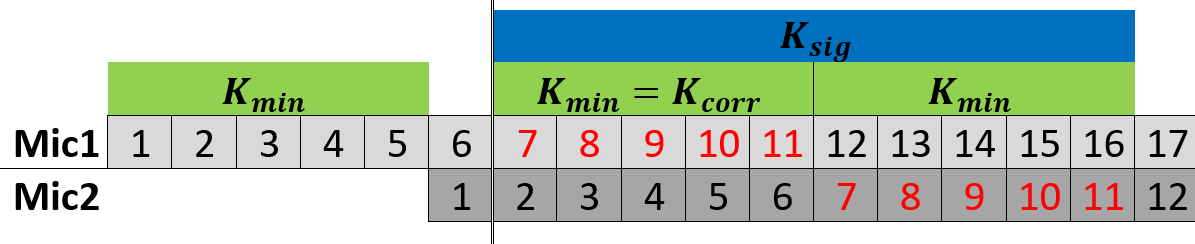
\includegraphics[width=0.4\textwidth]{Korrelation2}
\caption{Signalaufbau, anhand des Extremfalls mit maximaler Signalverschiebung}\label{fig:Korrelation2}
\end{figure}

Der Aufbau der  Signale anhand der genannten Bedingungen ist in Abbildung\ref{fig:Korrelation2} bildlich dargestellt. 
Es wird dabei der Extramfall mit einer maximalen Signalverschiebung (hier 5 ELmente) betrachtet. Würde ein Herrausschneiden der Signale (doppelte Linie) vor dem 5. Element gemacht werden, würden die entsprechenden Signale des zweiten Microfons abgeschnitten werden. Auch eine Verkürzung der Hautsignallänge (blau) würde zu einem Informaitonsverlust führen, da die Betrachtete Korrelationsfolge (rot) nicht mehr komplett im Signal2 enthalten wäre.\\
Oben beschriebene Bedingungen sind in Abbildung sind dann gültig, wenn sich das Moskito in einem Raum der nicht auf den Mikrofonraum von $1m x 1m x 1m$ begrenzt ist befinden kann.
Falls die Begrenzung auf den Mikrofonraums gilt, sollte eine Signallänge von $K_{corr}$ ausreichend sein. Bei der Begrenzung sind obige Bedingungen allerdings nicht hinderlich, sie sollten sogar zu einer höhren Genauigkeit führen. Daher wurden obige Bedinungen gewählt um den Raum des Moskitos zu erweitern.


\subsection{Untersuchung der Annahmen} \label{sec:Untersuchung}

